% TeXplates/Mathematics.tex
% v0.8.0
% https://github.com/HoyanMok/TeXplates
\documentclass[openany, a5paper]{book} 
% \documentclass{ctexbook} 如果用中文
% \documentclass[10pt,a4paper]{ctexart}  字体大小和纸张大小,默认分别为10pt和letterpaper
% 五号 = 10.5pt,小四=12pt,四号=14pt
% 其他可选参量如twocolumn, 两行排版

\usepackage{../TeXplatesMathematics}
\addbibresource{vonNeumannAlgebra.bib} % 把这里改成实际的文件名

% 文章标题页信息:
\title{von Neumann Algebras}
\author{Hoyan Mok}
\date{\today} % 自动生成日期
\titlepic{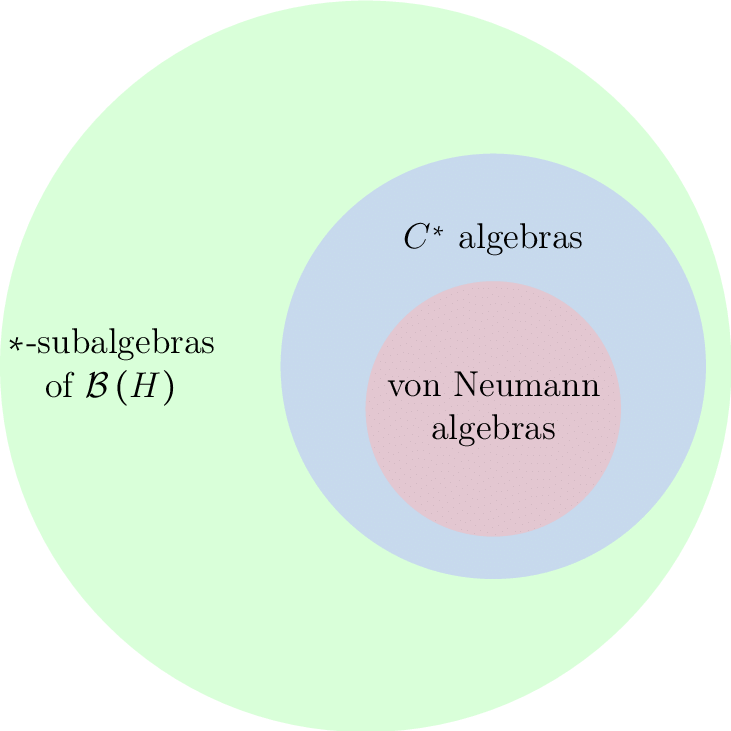
\includegraphics[width=.8\textwidth]{Diagram-to-show-relationship-between-B-H-C-algebras-and-von-Neumann-Algebras.png}}

\begin{document}
\pagenumbering{Alph}
\maketitle % 打印标题
\frontmatter
\chapter{Preface}

$\mathcal H$ means a Hilbert space by default.
If not specified, the base field is $\mathbb K = \mathbb R$ or $\mathbb C$.


\tableofcontents

\mainmatter
\chapter{Operators on Hilbert Spaces}
\section{Topologies on Spaces of Operators}

\begin{definition}[Topology generated by semi-norms]%
	\label{def: topology generated by semi-norms}
	Let $V$ be a vector space over $\mathbb K$.
	If $\{\|\dummy\|_i\}_{i \in I}$ is a family of seperated seminorms on $V$, 
	where ``seperated'' means that
	\begin{equation}
		\forall v \in V,\;
		\exists i_0 \in I,\;
		v \neq 0 \to \|v\|_{i_0} \neq 0,
	\end{equation} 
	then the \indexbf{topology generated by $\{\|\dummy\|_i\}_{i \in I}$} is the unique Hausdorff topology on $V$ s.t.\ 
	\begin{equation}
		\forall \langle v_n\rangle \in V^\mathbb N,\quad
		v_n \to v \in V \IFF \forall i \in I, \; \|v_n - v\|_i \to 0.
	\end{equation}
\end{definition}

The locally convexity is given by the the balanced local base
\begin{equation}
	\left\{
	\left\{v \in V \middle| \bigwedge_{k \in n} \|v\|_{i_k} < \varepsilon_k\right\}
	\middle|
	n \in \mathbb N_+, \; \forall k \in n,\,\varepsilon_k \in \mathbb R_+
	\right\}.
\end{equation}



\begin{theorem}[Continuous linear functionals on a locally convex space]
	Let $V$ be locally convex, with topology generated by $\{\|\dummy\|_i \mid i \in I\}$.
	A linear functional $f \in V^*$ is continuous \emph{iff}
	\begin{equation}
		\begin{gathered}
			\exists C \in \mathbb R_+,\; \exists n \in \mathbb N_+,\;\exists \{i_k \mid k \in n\} \subset I,\;\forall v \in V,
			\\
		|f(v)| \leq C \max_{k \in n} \|v\|_{i_k}.
		\end{gathered}
	\end{equation}
\end{theorem}

\begin{definition}[Strong-operator topology]%
	\label{def: strong-operator topology}
	Let $\mathcal H$ be a Hilbert space. 
	The \indexbf{strong-operator topology} (\indexbf{SO}) on the space of all bounded operators $B(\mathcal H)$ is the locally convex topology generated by the seminorms $\|\dummy\|_x$ ($x \in \mathcal H$), defined as
	\begin{equation}
		\begin{aligned}
		\|\|_x \colon
		B(\mathcal H) &\to \mathbb R
		\\
		T &\mapsto  \|Tx\|.
		\end{aligned}
	\end{equation}
\end{definition}

In SO topology, $T_n \to T$ iff $\forall x \in \mathcal H$, $\|T_n x - Tx\| \to 0$.

\begin{definition}[Weak-operator topology]%
	\label{def: weak-operator topology}
	The \indexbf{weak-operator topology} (\indexbf{WO}) on the space $B(\mathcal H)$ is the locally convex topology generated by the seminorms $\|\dummy\|_{x, y}$ ($x, y \in \mathcal H$), defined as
	\begin{equation}
		\begin{aligned}
		\|\|_{x, y} \colon
		B(\mathcal H) &\to \mathbb R
		\\
		T &\mapsto  |\langle Tx, y \rangle|.
		\end{aligned}
	\end{equation}
\end{definition}

In WO topology, $T_n \to T$ iff $\forall x, y \in H$, $\langle T_n x, y \rangle  \to \langle Tx, y \rangle$.
If $T_n \to T$ in SO topology, then it is true also in WO topology.

\begin{theorem}\label{thm: SO closure equals WO closure for convex set}
	Let $\mathscr S$ be a convex subset of $B(\mathcal H)$.
	The WO closure of $\mathscr S$ coincides with the SO closure of $\mathscr S$.
\end{theorem}


\chapter{Von Neumann Algebras}
\section{Von Neumann Algebras}
\begin{definition}[Von Neumann algebra]
	A $C^*$-subalgebra $\mathscr A$ of $B(\mathcal H)$ is called a \indexbf{von Neumann algebra} if $\mathscr A$ is closed in the SO topology.
\end{definition}

By Theorem~\ref{thm: SO closure equals WO closure for convex set}, a $C^*$-subalgebra $\mathscr A$ is a von Neumann algebra iff $\mathscr A$ is closed in the WO topology.

\section{Existence of Projections}

Recall that a projection is an element $p \in \mathscr A$ s.t.\ $p^2 = p = p^*$, where $\mathscr A$ is a $C^*$-algebra.



\appendix
\renewcommand{\theequation}{\Alph{chapter}-\arabic{equation}}
\chapter{Appendix}

\backmatter
\nocite{*} % 这个表示列出所有没有在文中被引用的参考文献
\printbibliography[heading=bibliography, title={Bibliography}]

\indexprologue{Here listed the important symbols used in this notes.}
\printindex[symbol]

\printindex

\end{document}